\subsection{Period 1: Stable detached haze Layer during the Northern Winter (2004-2008) - $L_s=\ang{300}-\ang{340}$}

At its arrival in the Saturnian system in 2004, Cassini observed a single detached haze layer at 500 km
(Fig.~\ref{fig:dhl_2004_2008}a) similar to the one observed at 350 km by Voyager 24 years before
\citep{Smith1981}. At that moment, we were two years after the winter solstice in the northern hemisphere, at $L_s=\ang{300}$.
In the southern hemisphere, the haze layer is completely detached from the main haze layer. The haze extinction is at least
one order of magnitude smaller inside the depleted zone (470 km) than in the main and the detached haze layers (below 450 and
at 500 km respectively). Between the equator and up to about \ang{60}N it presents only a local depletion in extinction
of a factor 10. There, the separation with the main haze is not as neat as in the south, but is still significant to
defined a detached haze layer.
The altitude of the depletion zone decreases by about 50 km between latitude \ang{30}N  and \ang{60}N.
The detached haze layer merges with the polar hood beyond \ang{60}N. This description of the detached haze layer at
the beginning of Cassini mission is very consistent with the results obtained from stellar occultation in 2003 \citep{Sicardy2006}.
The detached haze layer is quite stable in shape and set at a constant altitude, with a maximum of extinction
at $500 \pm 20$ km. The top of the main haze layer is located around $450 \pm 20$ km below \ang{30}N and drops
by 50 km between \ang{30} and \ang{60}N.

\begin{figure*}[!ht]
    \centering
    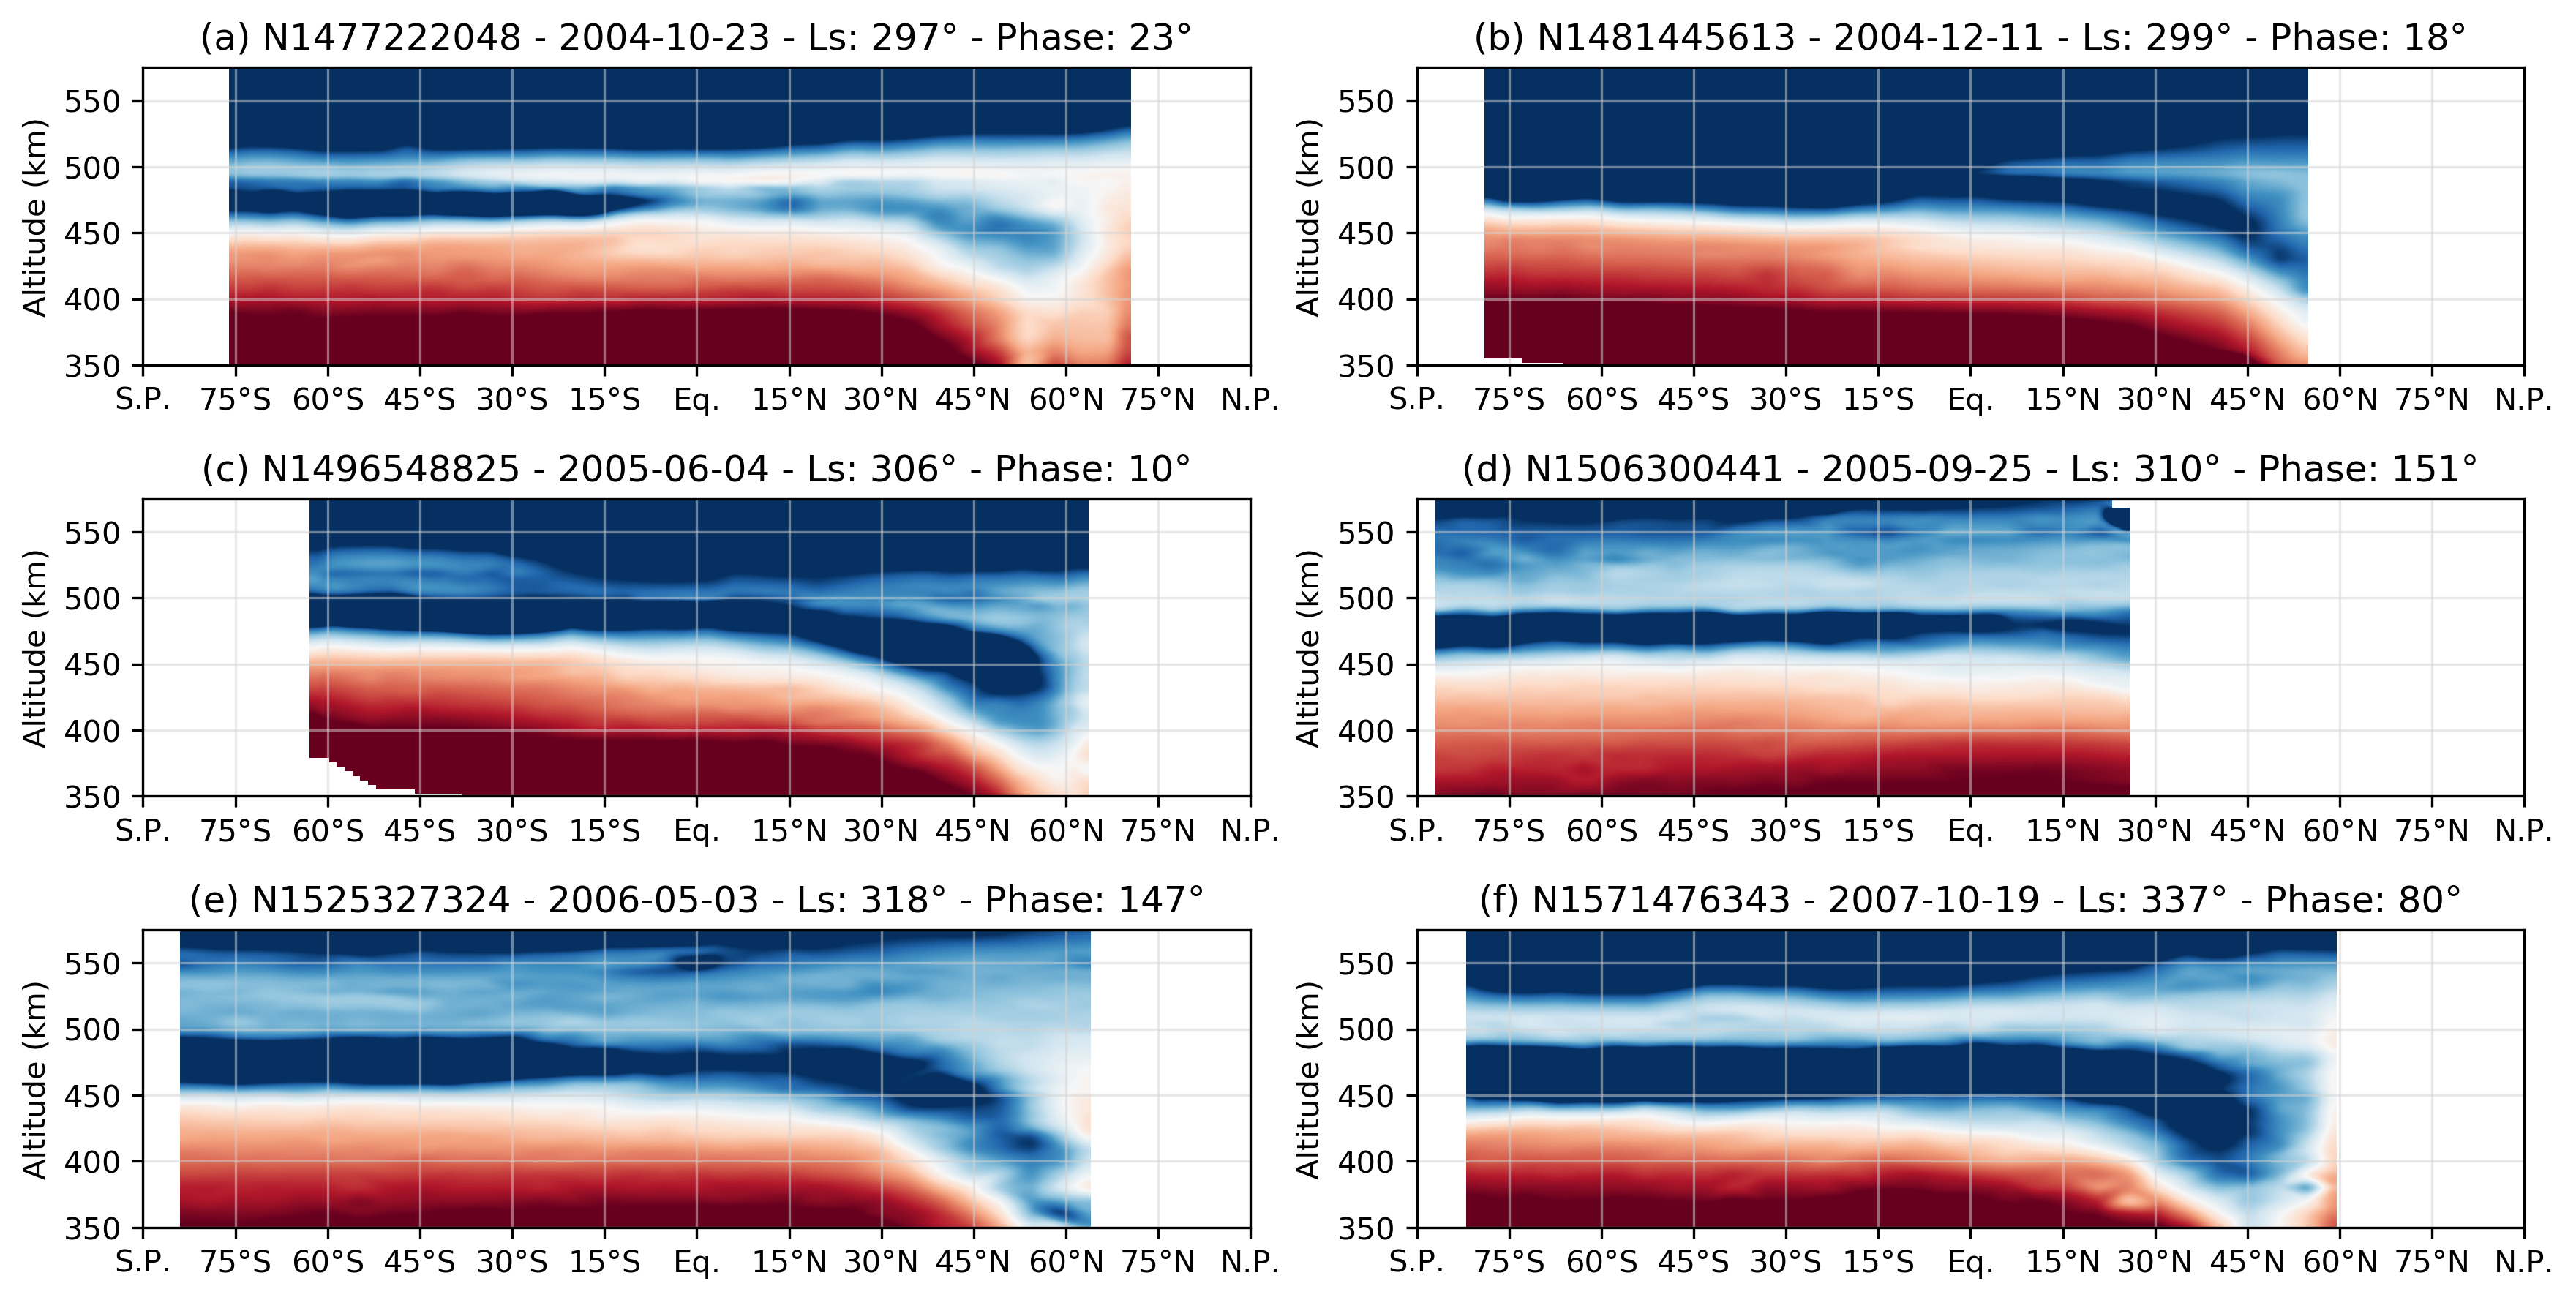
\includegraphics[width=\textwidth]{Fig/Lat_beta-2004_2008.png}
    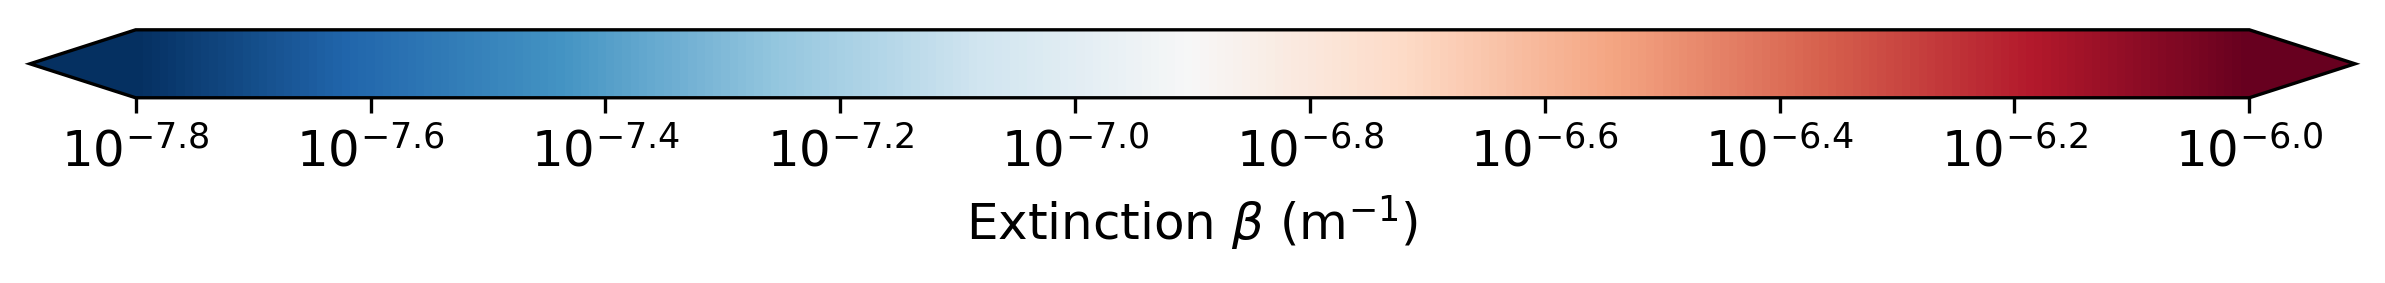
\includegraphics[width=.5\textwidth]{Fig/Extinction_colorbar.png}\vspace{-.3cm}
    \caption{Latitudinal haze extinction profile ($\beta$) retrieved for 6 images taken between 2004 and 2008
    ($L_s=\ang{300}-\ang{340}$) showing a stable DHL at $500 \pm 20$ km.
    The color schema extent is fixed for all the figures to make direct comparison
    between the different panels. The seasonal solar longitude ($L_s$) and the observation phase angle are
    also provided in each caption.}
    \label{fig:dhl_2004_2008}
\end{figure*}

However, there are noticeable variations in haze extinction. During several months, the
detached haze remained similar than for the first visit, but in December 2004 (Fig.~\ref{fig:dhl_2004_2008}b),
the detached haze layer extinction was found a factor of 10 lower than previously at almost all latitudes southern
of \ang{30}N, and about half a decade above \ang{30}N. The polar hood and the main haze are not affected by this decrease.
In the following observations, (Fig.~\ref{fig:dhl_2004_2008}c, d and e),
the detached haze was partially restored, but not with the same amount of extinction as before. Only observations in
2007 (Fig.~\ref{fig:dhl_2004_2008}f) show extinctions in the detached haze layer comparable to those before
the decrease. We note that the decrease of extinction below 370 km in the polar hood above \ang{50}N
(Fig.~\ref{fig:dhl_2004_2008}e) is due to an artefact of the inversion process. The stability of the large scale
structure of the detached haze layer is related to the steady state of the large scale circulation during all the winter.
The observation of October 2007 (Fig.~\ref{fig:dhl_2004_2008}f) is the last view that we have of this stable state
before the seasonal turnover.

During this period, the detached haze also has a strong layering with, at some latitudes, distinct decks which are not
continuous and rather appears as a foliation. This feature is more pronounced in some observations, for instance from
June 2005 to May 2006, but does not shows up in October 2007, except marginally beyond \ang{30}N. The foliated detached
haze layer has a larger geometrical thickness than before December 2004. This foliation is likely to be produced by a
specific large scale circulation that can last several terrestrial months to one year.

% NOTE: [PR] We should really check that the apparent difference in geometric thickness of the DHL is not due to something else, as for instance, the phase angle. It could be due to a real effect of some aerosols above the DHL which scatter in a different way than aerosols in DLH itself. Or it could be due to a deconvolution effect that could differ depending on the appearance of Titan as a full disk or a crescent...

As we will see in the \textbf{section 4}, the detached haze layer exhibits some longitudinal or diurnal variabilities
that prevents us to discuss minor features observed in single images in too much details. The small scale features
could depends on the local short term dynamics.
